% contient une explication du fonctionnement du Mip Map et du Rip Map, et des schémas explicatifs. En bref, un résumé de l'article de Williams
% parler éventuellement de la méthode naïve, ou d'autres méthodes actuelles qui ne fonctionnent pas
  Afin de traiter des homographies plusieures méthodes ont été développées. Cette partie présente de manière non-exhaustive les méthodes déjà existantes (méthode naïve, Mipmap et Ripmap). Elles seront comparées avec notre nouvelle méthode dans les expériences.


\ssse{Méthode naïve}

On peut imaginer une méthode naïve : on utilise simplement la formule de l'homographie. Ainsi pour chaque point de l'image d'arrivée, on peut calculer la zone de l'image de départ correspondant via l'homographie inverse. On se heurte à un premier problème, en effet on ne tombe pas précisément sur un pixel de l'image de départ mais entre plusieurs pixels. 

On peut par exemple prendre la couleur du pixel le plus proche. Il apparait alors de l'\emph{aliasing} : en effet les pixels qu'on a modélisés par des points ont visuellement une épaisseur. Ainsi quand il y a localement un \emph{zoom-out} il faut moyenner l'image de départ sur une certaine zone.

%image aliasé à fond

\begin{figure}[h!]
\centering
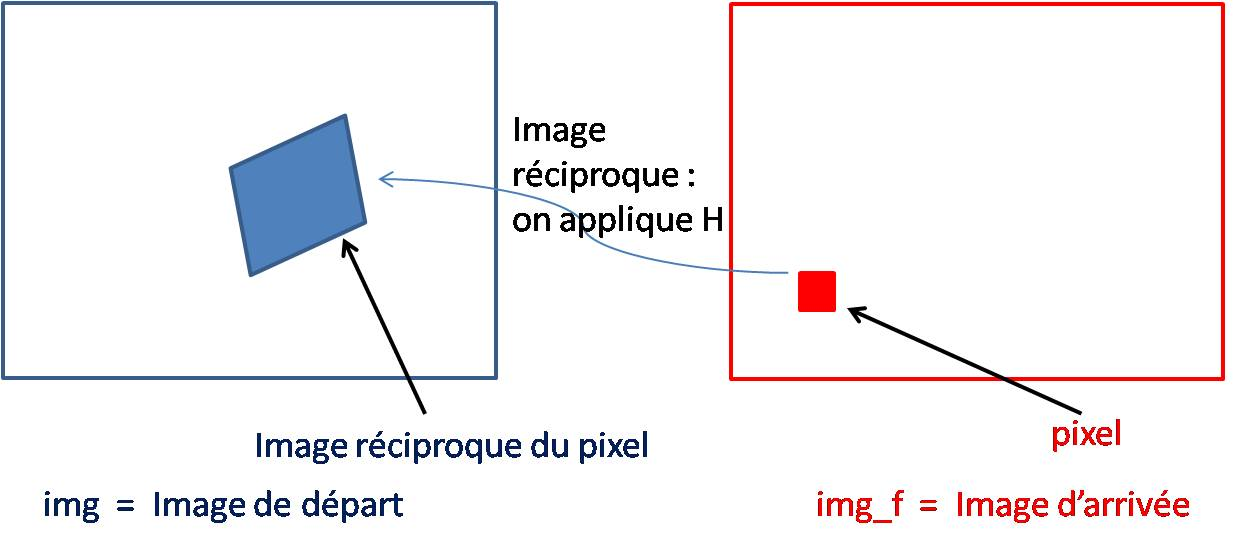
\includegraphics[scale=0.5]{imagereciproque.jpg}
\caption{Image réciproque d'un pixel}
\end{figure}

En pratique on utilise plutôt le Mipmap. C'est une méthode utilisée en texturing, présentée par Williams en 1983 \cite{williams1983pyramidal}.

\ssse{Présentation du Mipmap}

Le principe du Mipmap est de précalculer des coefficients qui représentent des zones entières de l'image, pour pouvoir ensuite calculer en temps réel une homographie. 

Pour cela on choisit de supposer que l'image est carrée de taille une puissance de 2 (quitte à faire un premier zoom). On calcule ensuite la valeur de certains carrés de l'image de taille une puissance de 2.
Le Mipmap est donc représenté par une suite d'images chacune deux fois plus petite que la précédente. Ainsi c'est un suite de \emph{zoom-out} de l'image d'origine de facteur une puissance de 2.

\begin{figure}[h!]
\centering
\caption{Un exemple de Mipmap}
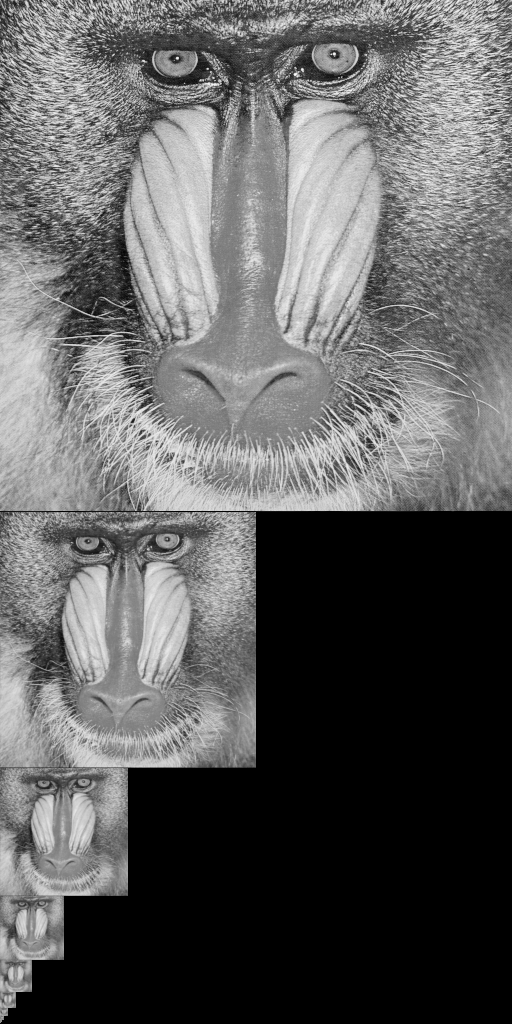
\includegraphics[scale=0.4]{MipMap_real} %scale=0.4 ça fait vachement petit, non ?
\end{figure}

Quand on cherche la valeur d'un pixel de l'image d'arrivée, on approche la zone de l'image de départ à laquelle il correspond à l'aide des différentielles de l'homographie inverse. On obtient alors un parallélogramme, qu'on essaye d'approcher avec des carrés. %ou qui s'approxime par des carrés

%image de parallélogramme avec les différentielles, avec au mieux schéma image de départ / arrivé qui explique la correspondance entre un pixel est un parallélogramme

On appelle distance d'un pixel la taille du carré choisi pour l'approximation (car plus un pixel est "loin", plus les carrés qui l'approchent sont grands). 

On suppose avoir une formule qui nous donne la distance d'un point quelconque. La géométrie du Mipmap ne permettant que des distances puissance de 2, on fait une approximation trilinéaire : 

\begin{itemize}
  \item d'une part, on fait une interpolation linéaire entre deux étages dont les profondeurs encadrent la distance.
  \item d'autre part, dans chaque étage du Mipmap, on fait une interpolation bilinéaire entre les quatre carrés qui encadrent le pixel.
\end{itemize}

\begin{figure}[h!]
\centering
\caption{Schéma d'interpolation trilinéaire}
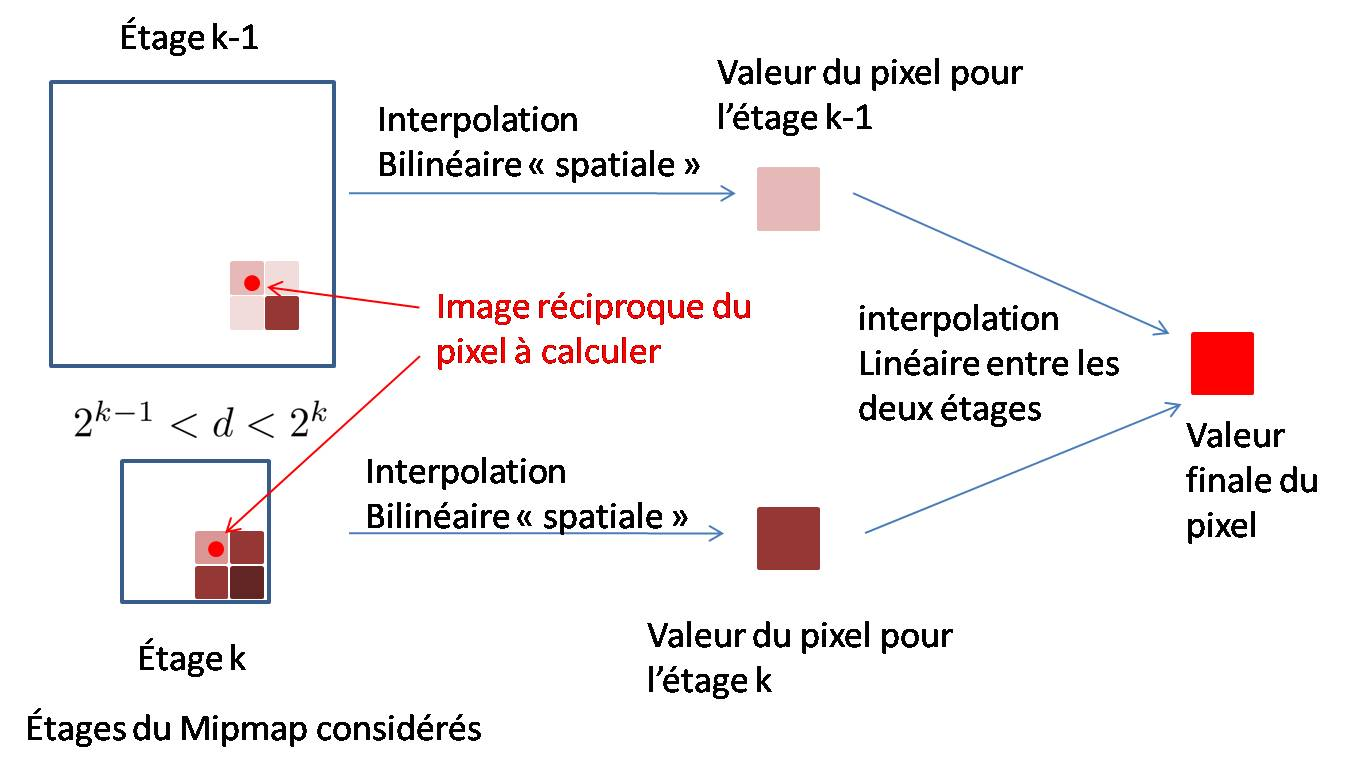
\includegraphics[scale=0.5]{intertrilineaire.jpg}
\end{figure}

\ssse{La fonction de distance}

Toutes les fonctions de distance dépendent de la différentielle de l'homographie inverse.
On note $(u,v)$ les coordonnées dans l'image d'origine et $(x,y)$ celles dans la fenêtre d'arrivée.

Le choix de la distance est crucial car si $d$ est trop grand, l'image est inutilement floutée (on parle d'\emph{over-blurring}), et si $d$ est trop petit l'image est aliasée.

Il est aisé de calculer les coefficients des dérivées partielles. On note $H$ l'homographie inverse.

%re image prgm, avec les dérivé partielle indiqués

% On a jugé de la performance des méthodes "à vue". On compte à terme l'évaluer sur des cosinus/sinus.

On note $\dd_{(x,y)} H$ la différentielle de $H$ en $(x,y)$.

On note $(u,v)=H(x,y)$.

\sssse{Méthode du déterminant}
$$D(x,y) = \sqrt{\det \txt{d}_{(x,y)} H}$$
Cette formule est justifiée car le déterminant de $\txt{d}_{(x,y)} H$ est l'aire du parallélogramme, donc un carré de côté $\sqrt{\det \txt{d}_{(x,y)} H}$ est de même aire que le parallélogramme qu'il approche.

\begin{figure}[h!]
\centering
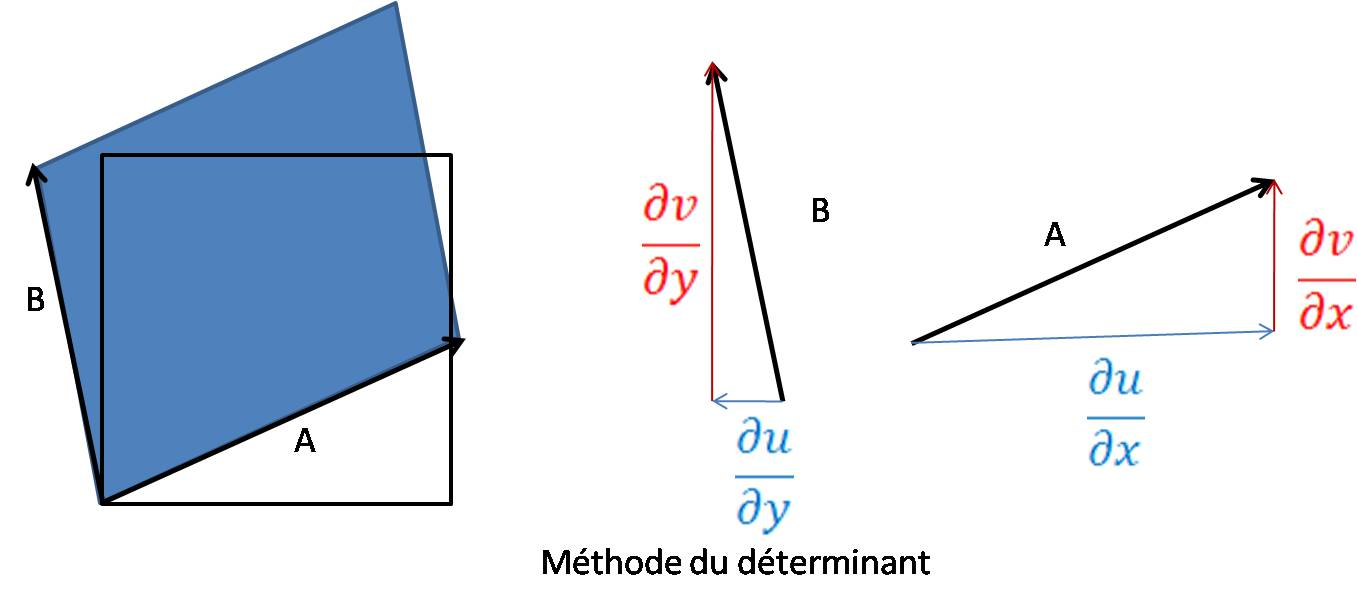
\includegraphics[scale=0.5]{methode_determinant.jpg}
\end{figure}


Le résultat est relativement satisfaisant.

%schéma avec un ârallélogramme et le carré correspondant

\sssse{Méthode du plus grand côté}
$$ D(x,y) = \max \left(\sqrt{\left(\frac{\dr u}{\dr x}\right)^2 + \left(\frac{\dr v}{\dr x}\right)^2},\sqrt{\left(\frac{\dr u}{\dr y}\right)^2 + \left(\frac{\dr v}{\dr y}\right)^2}\right)$$
On prend le plus grand côté du parallélogramme comme côté du carré. Cette formule viens d'un article de Heckbert \cite{heckbert1983texture}.
% On prend le plus grand côté du parallélogramme comme côté du carré \cite{heckbert1983texture}. Le résultat est bon.

\begin{figure}[h!]
\centering
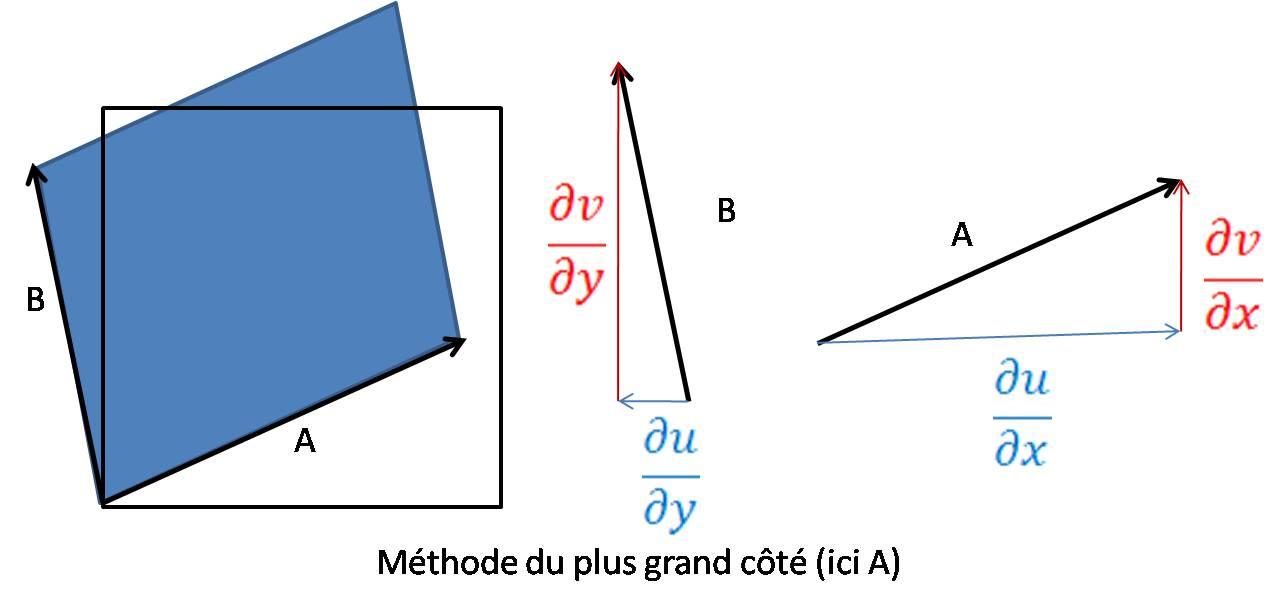
\includegraphics[scale=0.5]{methode_plus_grand_cote.jpg}
\end{figure}


Ce résultat est satisfaisant.

%schéma avec un ârallélogramme et le carré correspondant

\sssse{Méthode des diagonales}
$$D(x,y) = \max \left( \sqrt{\left(\frac{\dr v}{\dr x}-\frac{\dr  u}{\dr  x}\right)^2+\left(\frac{\dr v}{\dr y}-\frac{\dr  u}{\dr y}\right)^2}, \sqrt{\left(\frac{\dr u}{\dr x}+\frac{\dr  v}{\dr  x}\right)^2+\left(\frac{\dr u}{\dr y}+\frac{\dr  v}{\dr  y}\right)^2} \right)$$
On prend la plus grande diagonale du parallélogramme. Ici l'image est trop floue.

\begin{figure}[h!]
\centering
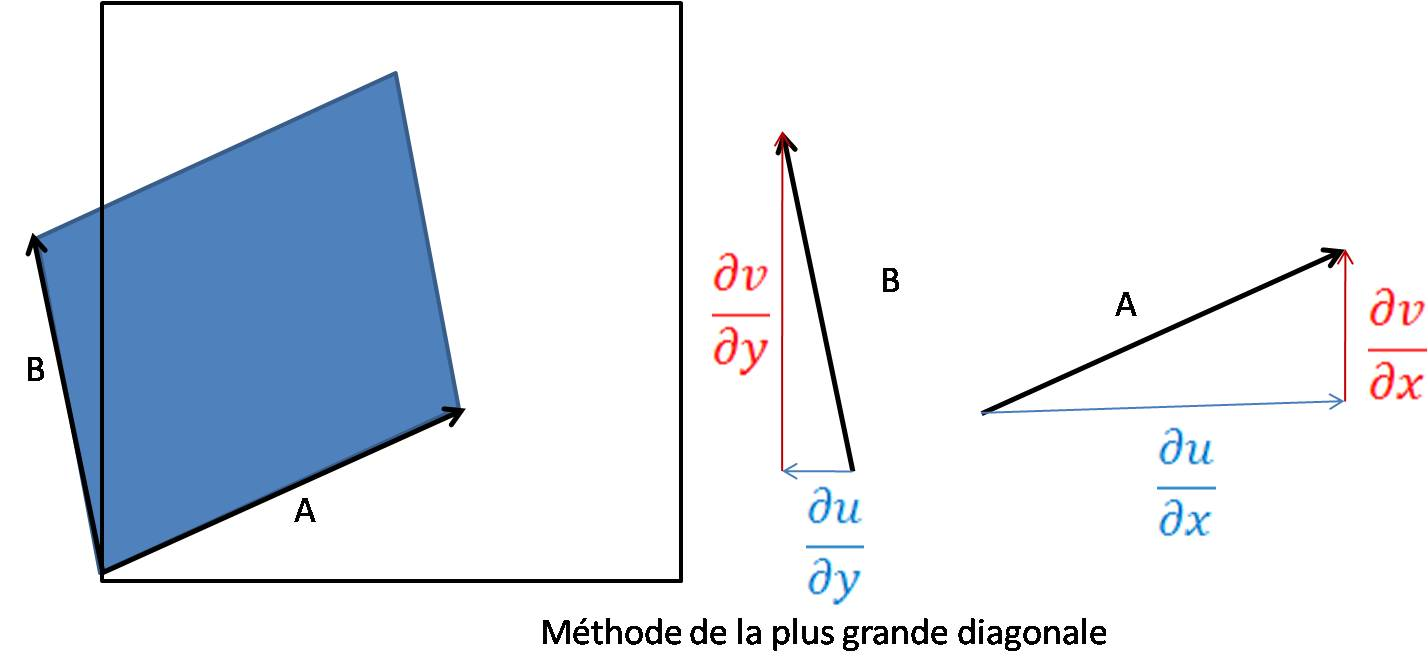
\includegraphics[scale=0.5]{methode_grande_diagonale.jpg}
\end{figure}

%schéma avec un parallélogramme et le carré correspondant

\sssse{Méthode des valeurs singulières}

On peut décomposer toute matrice $A$ en trois matrices $A = PDQ^{-1}$ où $P$ et $Q$ sont orthogonales et $D$ est diagonale.

Pour cela on diagonalise $AA^t$, et $A^tA$, on prend $P$ et $Q$ des vecteurs propres normalisés de ces matrices, et $D$ la racine de leur diagonalisée. Il faut veiller à ce que $P$ et $Q$ correspondent bien \cite{abdi2007singular}.

Les coefficients de $D$ sont appelés valeurs singulières de $A$. On prend $D(x,y)$ le maximum des deux valeurs singulières de $A$.


\begin{figure}[h!]
\centering
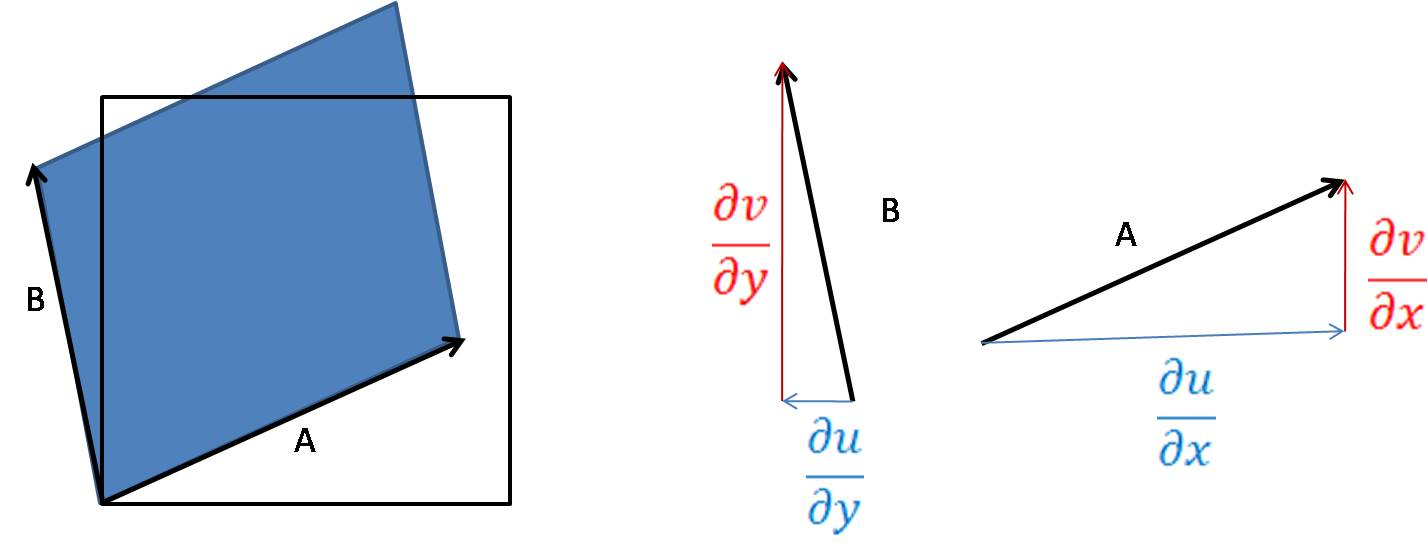
\includegraphics[scale=0.5]{methode_valeur_singuliere.jpg}
\end{figure}

On a une interprétation géométrique comme un mouvement de caméra de ces valeurs \cite{morel2009asift}.

\sssse{Conclusion}

Les méthodes du déterminant, du plus grand côté du parallélogramme et du maximum des valeurs singulières sont satisfaisantes.

On a une préférence pour le plus grand côté et la valeur singulière, en effet le déterminant semble introduire un peu plus d'\emph{aliasing}.

\ssse{Algorithme amélioré : Le Ripmap}

Une des grandes faiblesses du Mipmap est l'isotropie : il ne privilégie aucune direction. Ainsi si le parallélogramme à approcher est un rectangle très plat, il n'y a pas d'approximation raisonnable à l'aide d'un carré.

Pour tenter de résoudre ce problème on utilise un Ripmap \cite{akenine2008real}. C'est en fait un Mipmap où l'on a aussi calculé la moyenne des pixels de tous les rectangles dont les côtés sont des puissances de deux.

Ainsi la fonction de distance ne renvoie plus une seule valeur mais une pour chaque côté du rectangle. On réalise alors une interpolation quadrilinéaire (bilinéaire entre les étages et bilinéaire dans chacun d'eux).%bibilinéaire ? sérieusement ?



%un vrai ripmap, que je ferais moi
\begin{figure}[h!]
\centering
\caption{Un exemple de Ripmap}
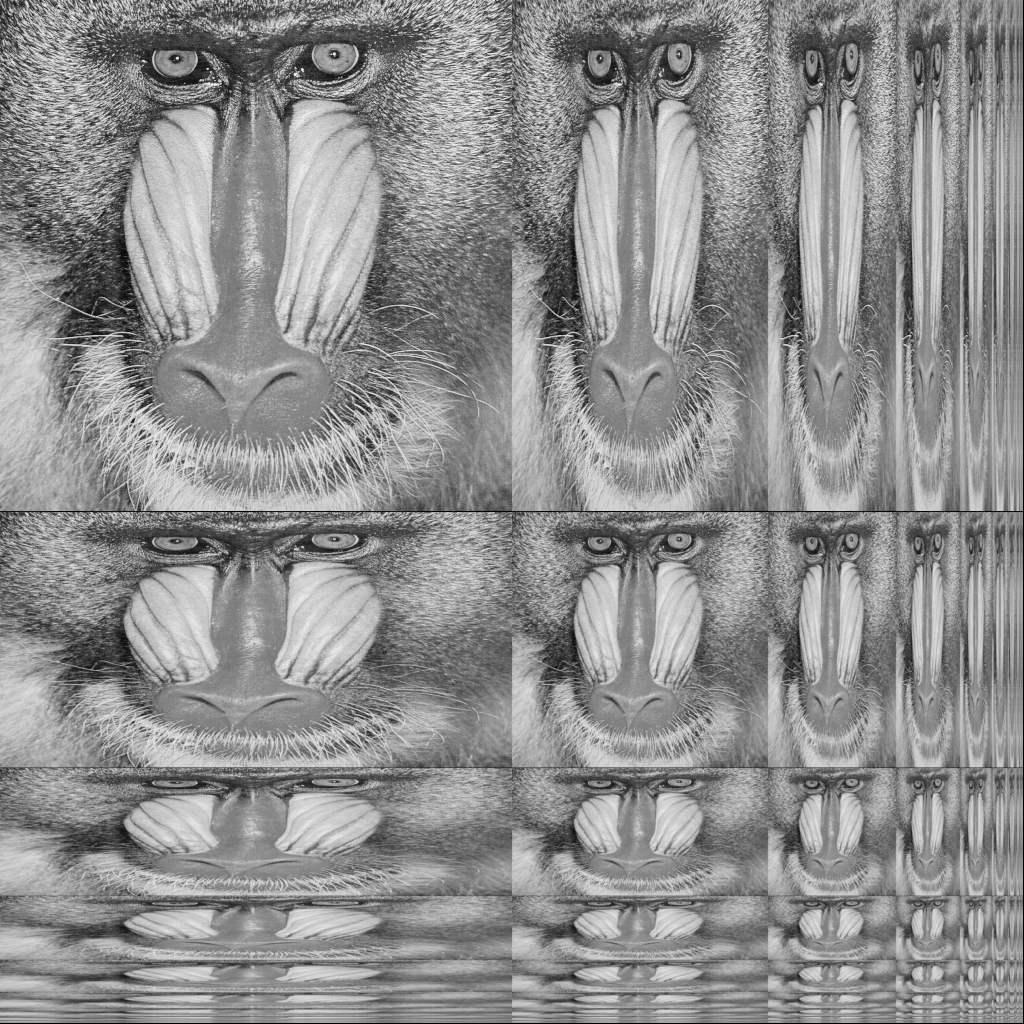
\includegraphics[scale=0.4]{Ripmap_real}
\end{figure}


%schéma d'interpolations pour le ripmap, avec 4 images est l'endroit ou le point tombe dans chacun
\begin{figure}[h!]
\centering
\caption{Schéma d'interpolation quadrilinéaire}
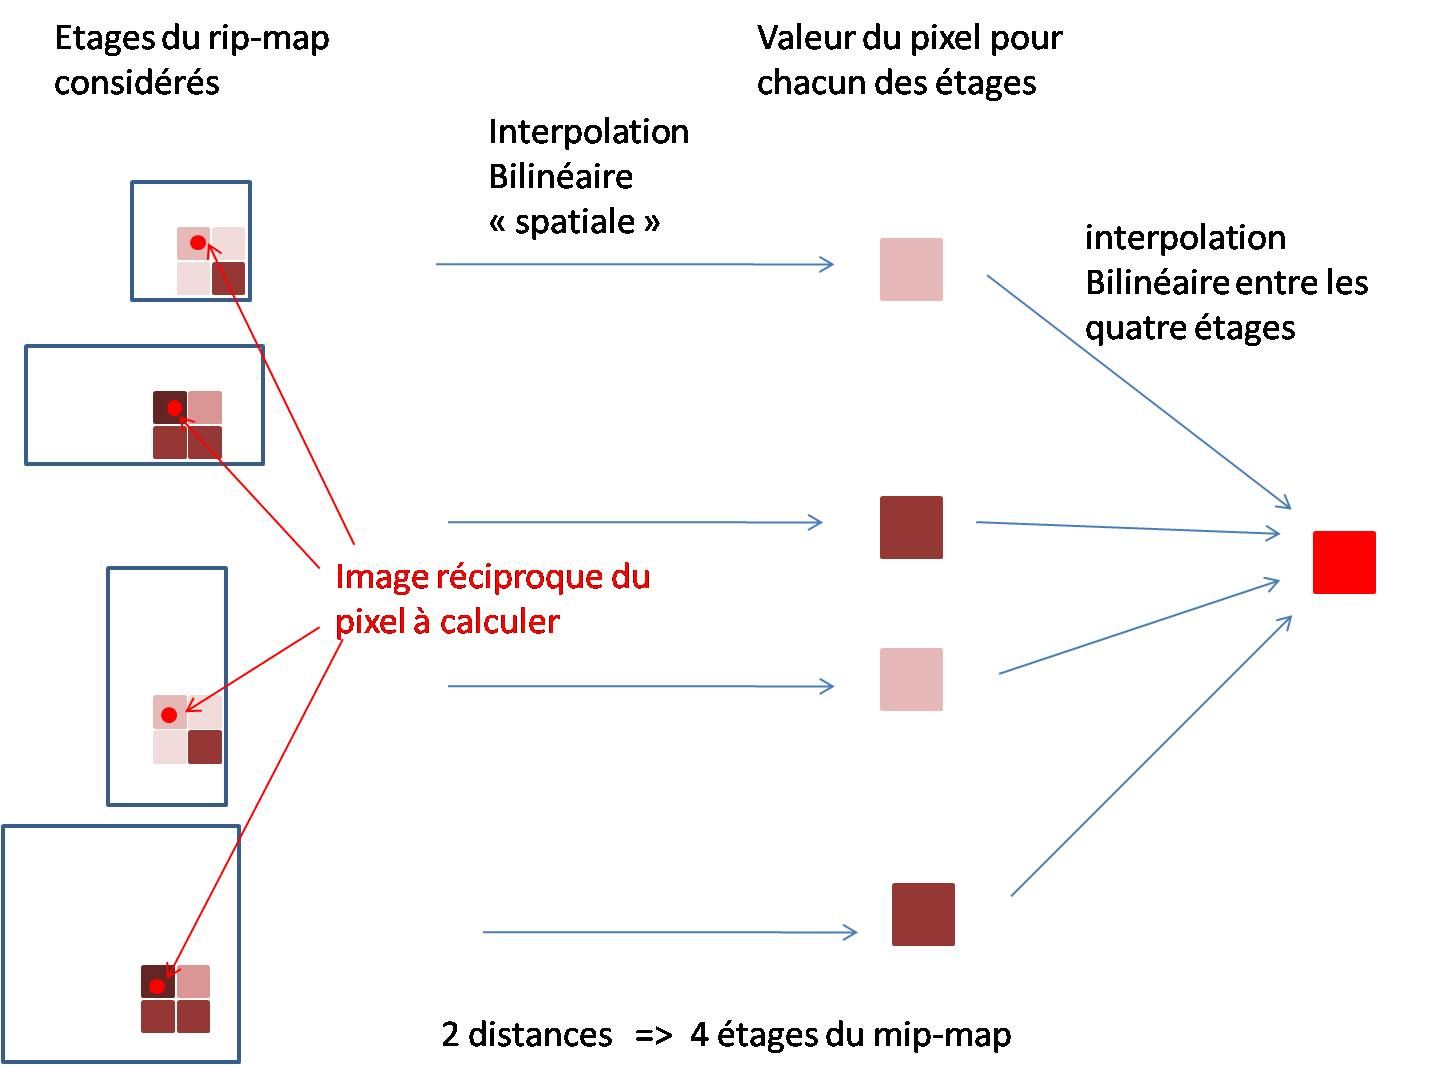
\includegraphics[scale=0.5]{interbibilineaire.jpg}
\end{figure}


On a utilisé le plus petit rectangle qui contient le parallélogramme. Ainsi la formule est :
$$D(x,y) = \left( \left|\frac{\dr u}{\dr x}\right|+\left|\frac{\dr u}{\dr y}\right|,\left|\frac{\dr v}{\dr x}\right|+\left|\frac{\dr v}{\dr y}\right|\right)$$
On a de plus décalé les points pour que le rectangle considéré soit bien celui qui contient le parallélogramme.

\begin{figure}[h!]
\centering
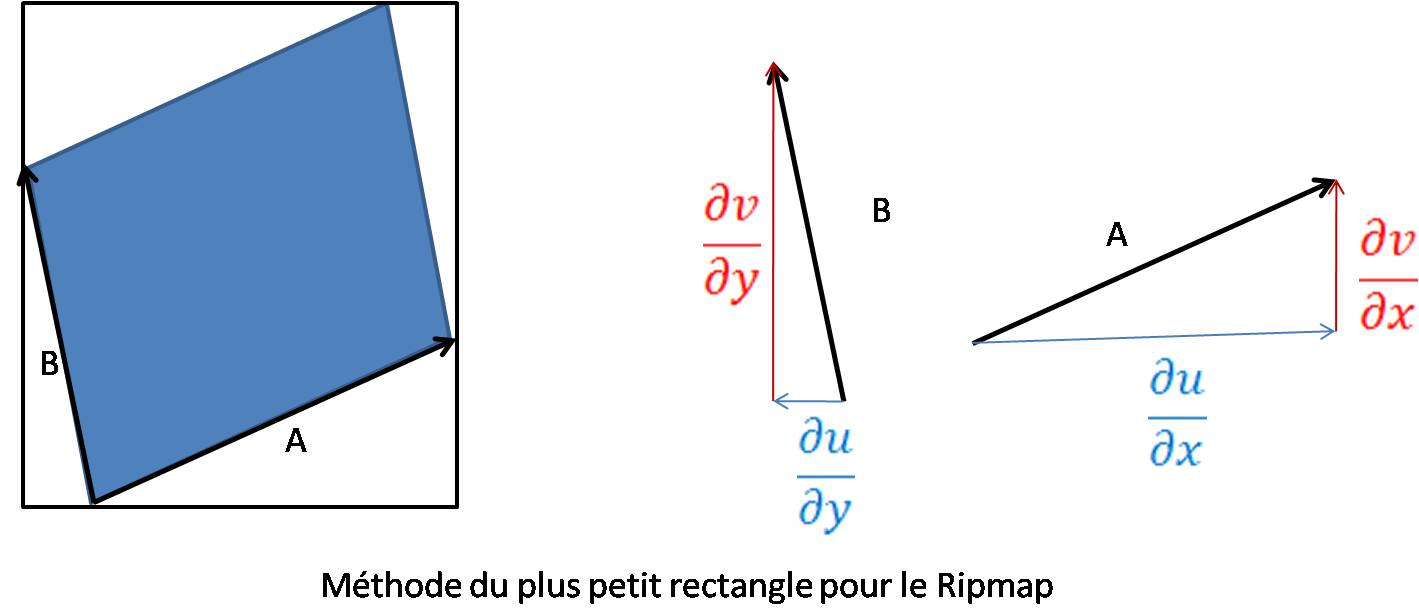
\includegraphics[scale=0.5]{methode_distance_ripmap.jpg}
\end{figure}

Cela améliore certes la méthode, mais ne résout pas par exemple le cas d'un rectangle fin en diagonale.
